% Chapter 3

\chapter{BACKGROUND AND MOTIVATION} % Write in your own chapter title
%

\section{REINFORCEMENT LEARNING}

%\im

Reinforcement Learning is a sub-domain of machine learning, in which a
learner or agent must find an optimal method to perform a specific
task when interacting with a dynamic environment. The agent is made to
learn from the experience it gains from said interaction. The actions
of the agent influence the environment, and thus also influences the
agent's future actions. Therefore the goal of an agent is to find the
optimal actions for the state it is in, with an objective of
maximizing net reward.
%
% \begin{figure}[hbt] 
% \begin{center}
% \includegraphics[scale=.40]{./figures/bddig}
% \caption{\label{fig:BDD}Binary Decision Diagram}
% \end{center}
% \end{figure}

An agent in the environment, in the state $s_{i} $, performs an action
$a_{i} $ using a policy $\pi$, to reach the state $s_{i+1} $, upon
which the agent collects a reward $r_{i} $. The policy $\pi$ is used
to take an action $a_{i} $ based on the value function at $s_{i+1} $,
so as to maximize its future rewards. The reward returned to the
model, based on its action, is then used as feedback to quantify the
agent's performance.
% \begin{figure}[hbt] 
% \begin{center} 
% \includegraphics[scale=.40]{./figures/BDD1}
% \caption{\label{fig:subBDD}A BDD with duplicated subBDDs.}
% \end{center}
% \end{figure}


%
% \begin{figure}[hbt] 
% \begin{center}
% \includegraphics[scale=.40]{./figures/subBDD}
% \caption{\label{fig:subBDDs1}After removal of duplicate $y$-node}
% \end{center}
% \end{figure}

% \begin{figure}[hbt] 
% \begin{center}
% \includegraphics[scale=.40]{./figures/BDD2}
% \caption{\label{fig:subBDD1}After removal of redundant $x$-decision point.}
% \end{center}
% \end{figure}

Most reinforcement learning problems can be formally defined as a
Markov Decision Process. That is, the problems can be defined
following the Markov Property: the transition probability and the
reward depend only on the current state $s_{i} $ and action $a_{i} $,
and are not influenced by the past states and actions.

%INCLUDE MARKOV EQN 

A key component of Reinforcement learning is the
exploration-exploitation problem. Exploration is the virtue
by which an agent is able to experience new states while
interacting with the environment, and exploitation is when
the agent is able to use its knowledge gained in prior
iterations to choose the optimal decision. During training it
is recommended that the agent explores a multitude of states,
to learn the alternative paths to the end goal, in order to
determine the optimal path. However it is also important to
monitor the exploration, to ensure that the agent does miss a
potentially optimal path.

\begin{figure}[H]
    \centering
    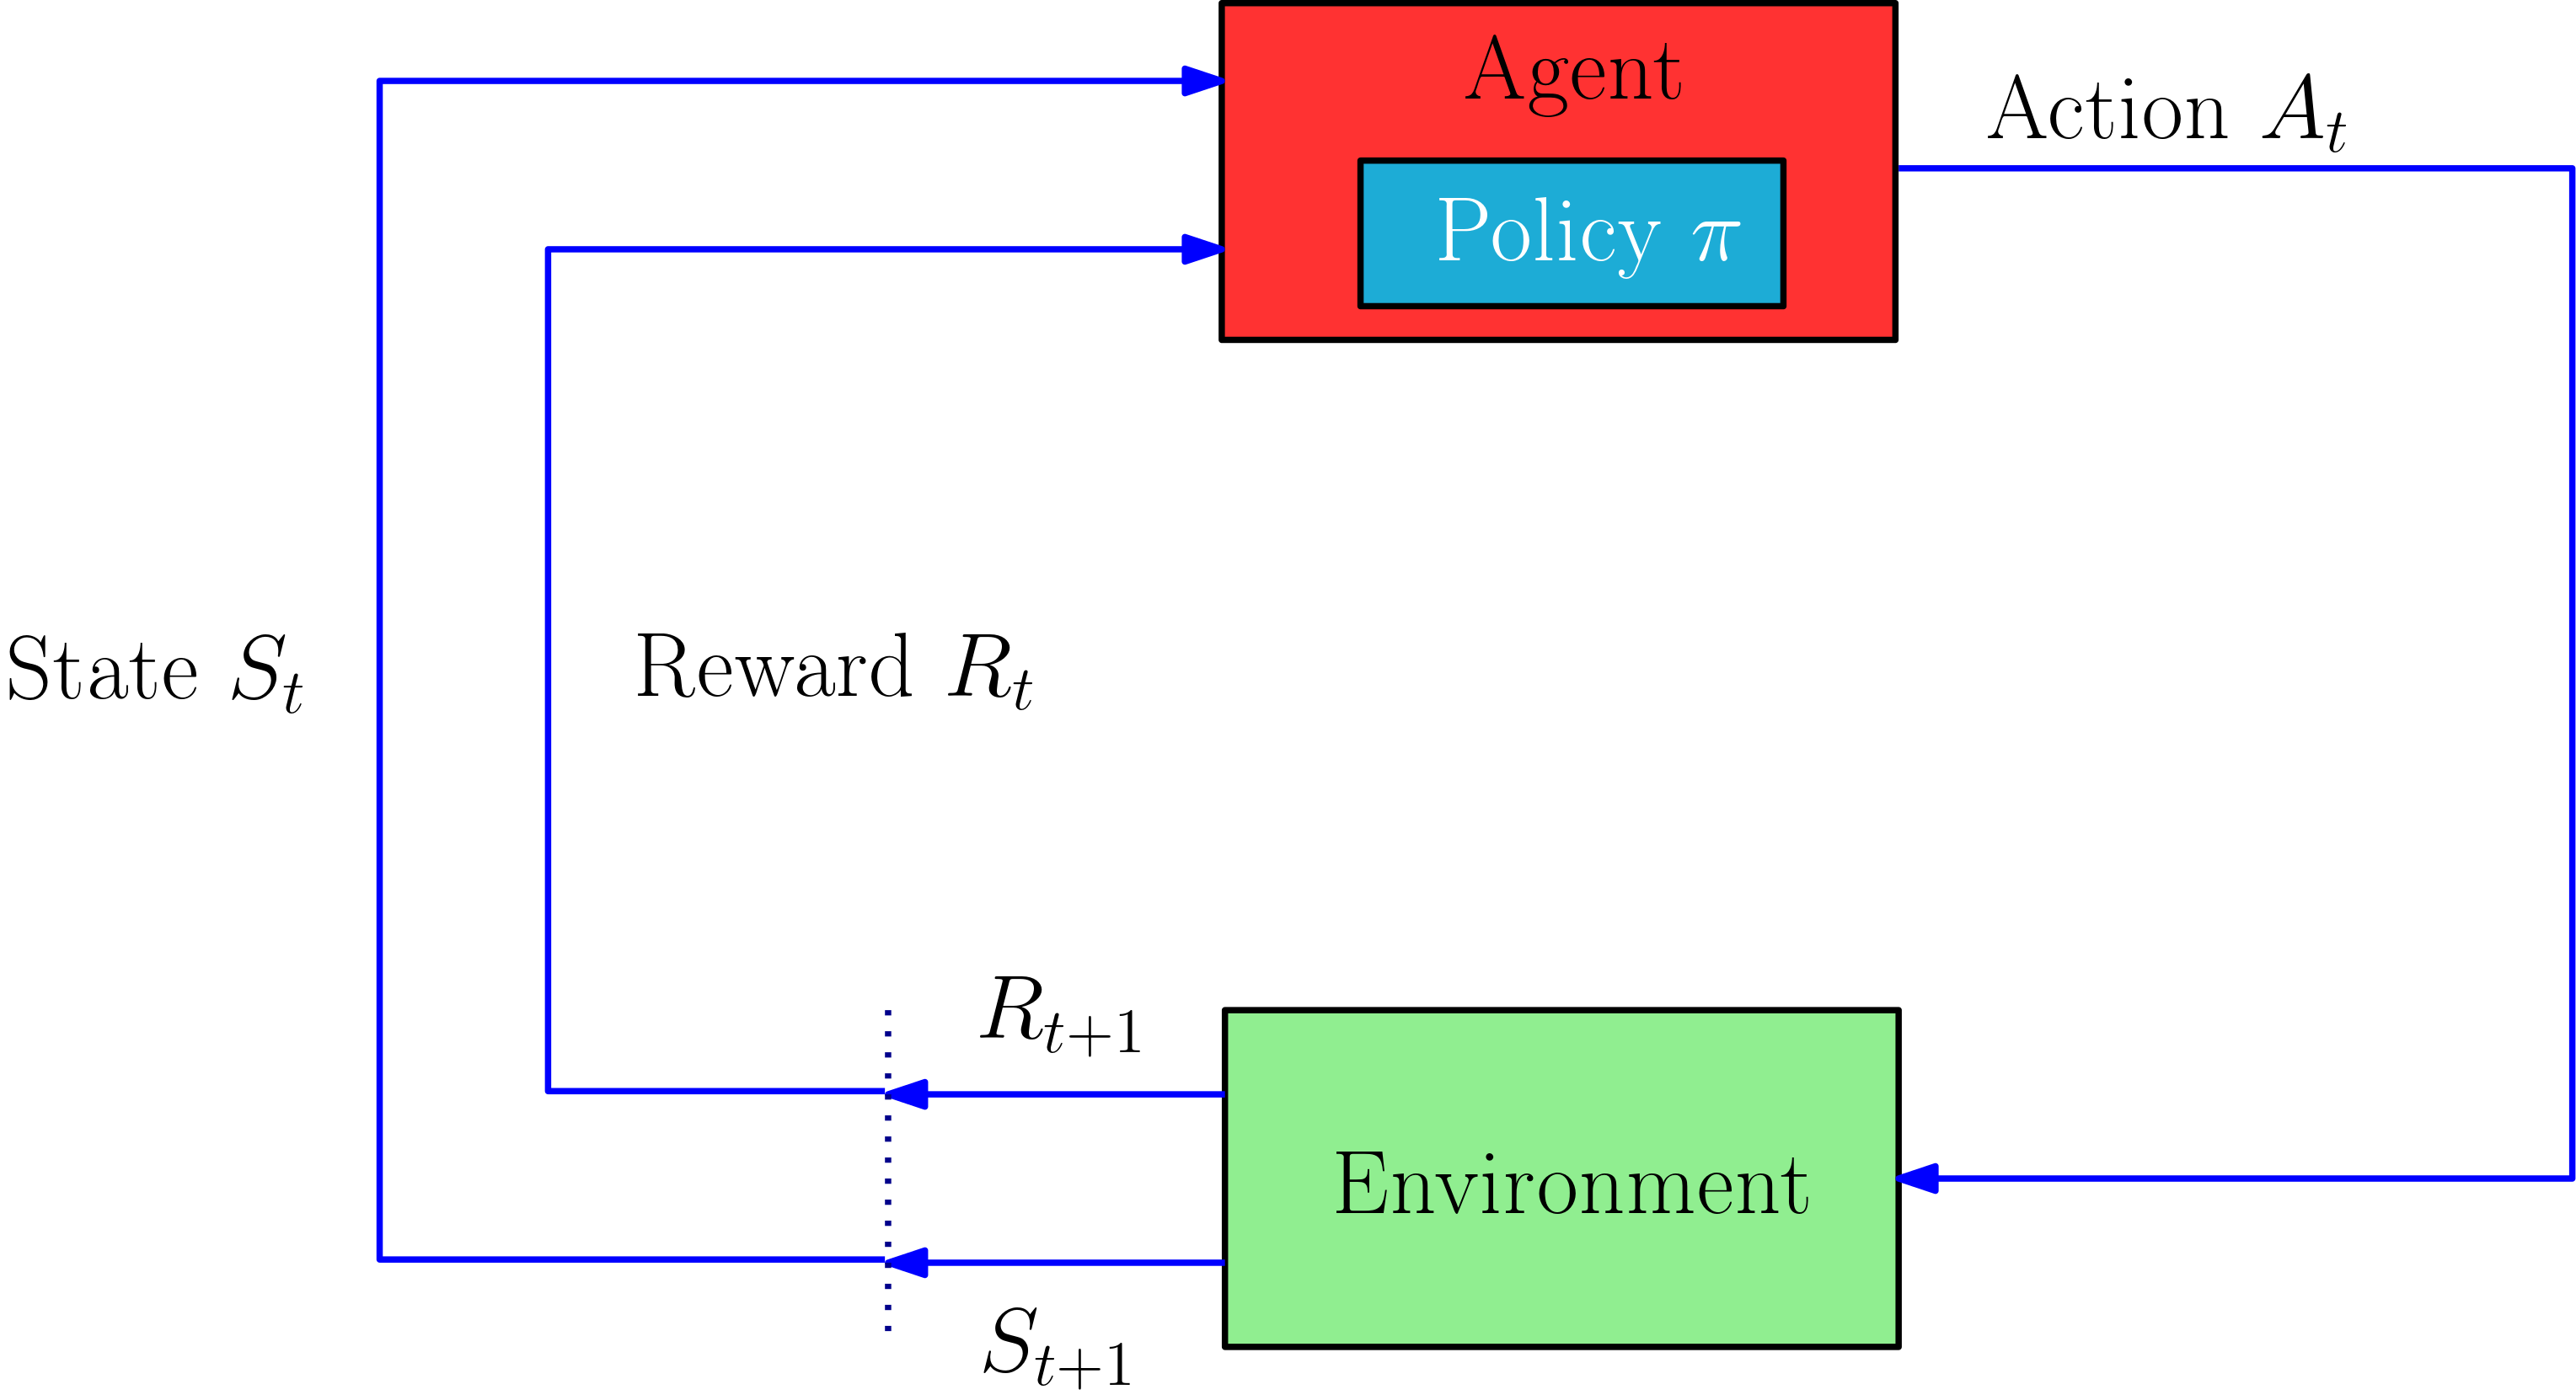
\includegraphics[width=0.9\textwidth]{images/rlv3.png}
    \caption{Reinforcement Learning}
    \label{fig:rl}
\end{figure}

% \begin{figure}[hbt] 
% \begin{center}
% \includegraphics[scale=.40]{./figures/bddig1}
% \caption{\label{fig:BDDD}A BDD where some boolean variables occur more than
% once on an evaluation path.}
% \end{center}
% \end{figure}

\subsection{DEEP REINFORCEMENT LEARNING}

We have already seen that in reinforcement learning, the
agent tries to learn a policy $\pi$ in order to maximize its
rewards. The policy $\pi$ is usually given by
$\pi(s\gets a)$, a function mapping states to actions. In
deep reinforcement learning, we use neural networks to
approximate the policy $\pi$, and other learnable functions
such as the value function.

\begin{figure}[H]
    \centering
    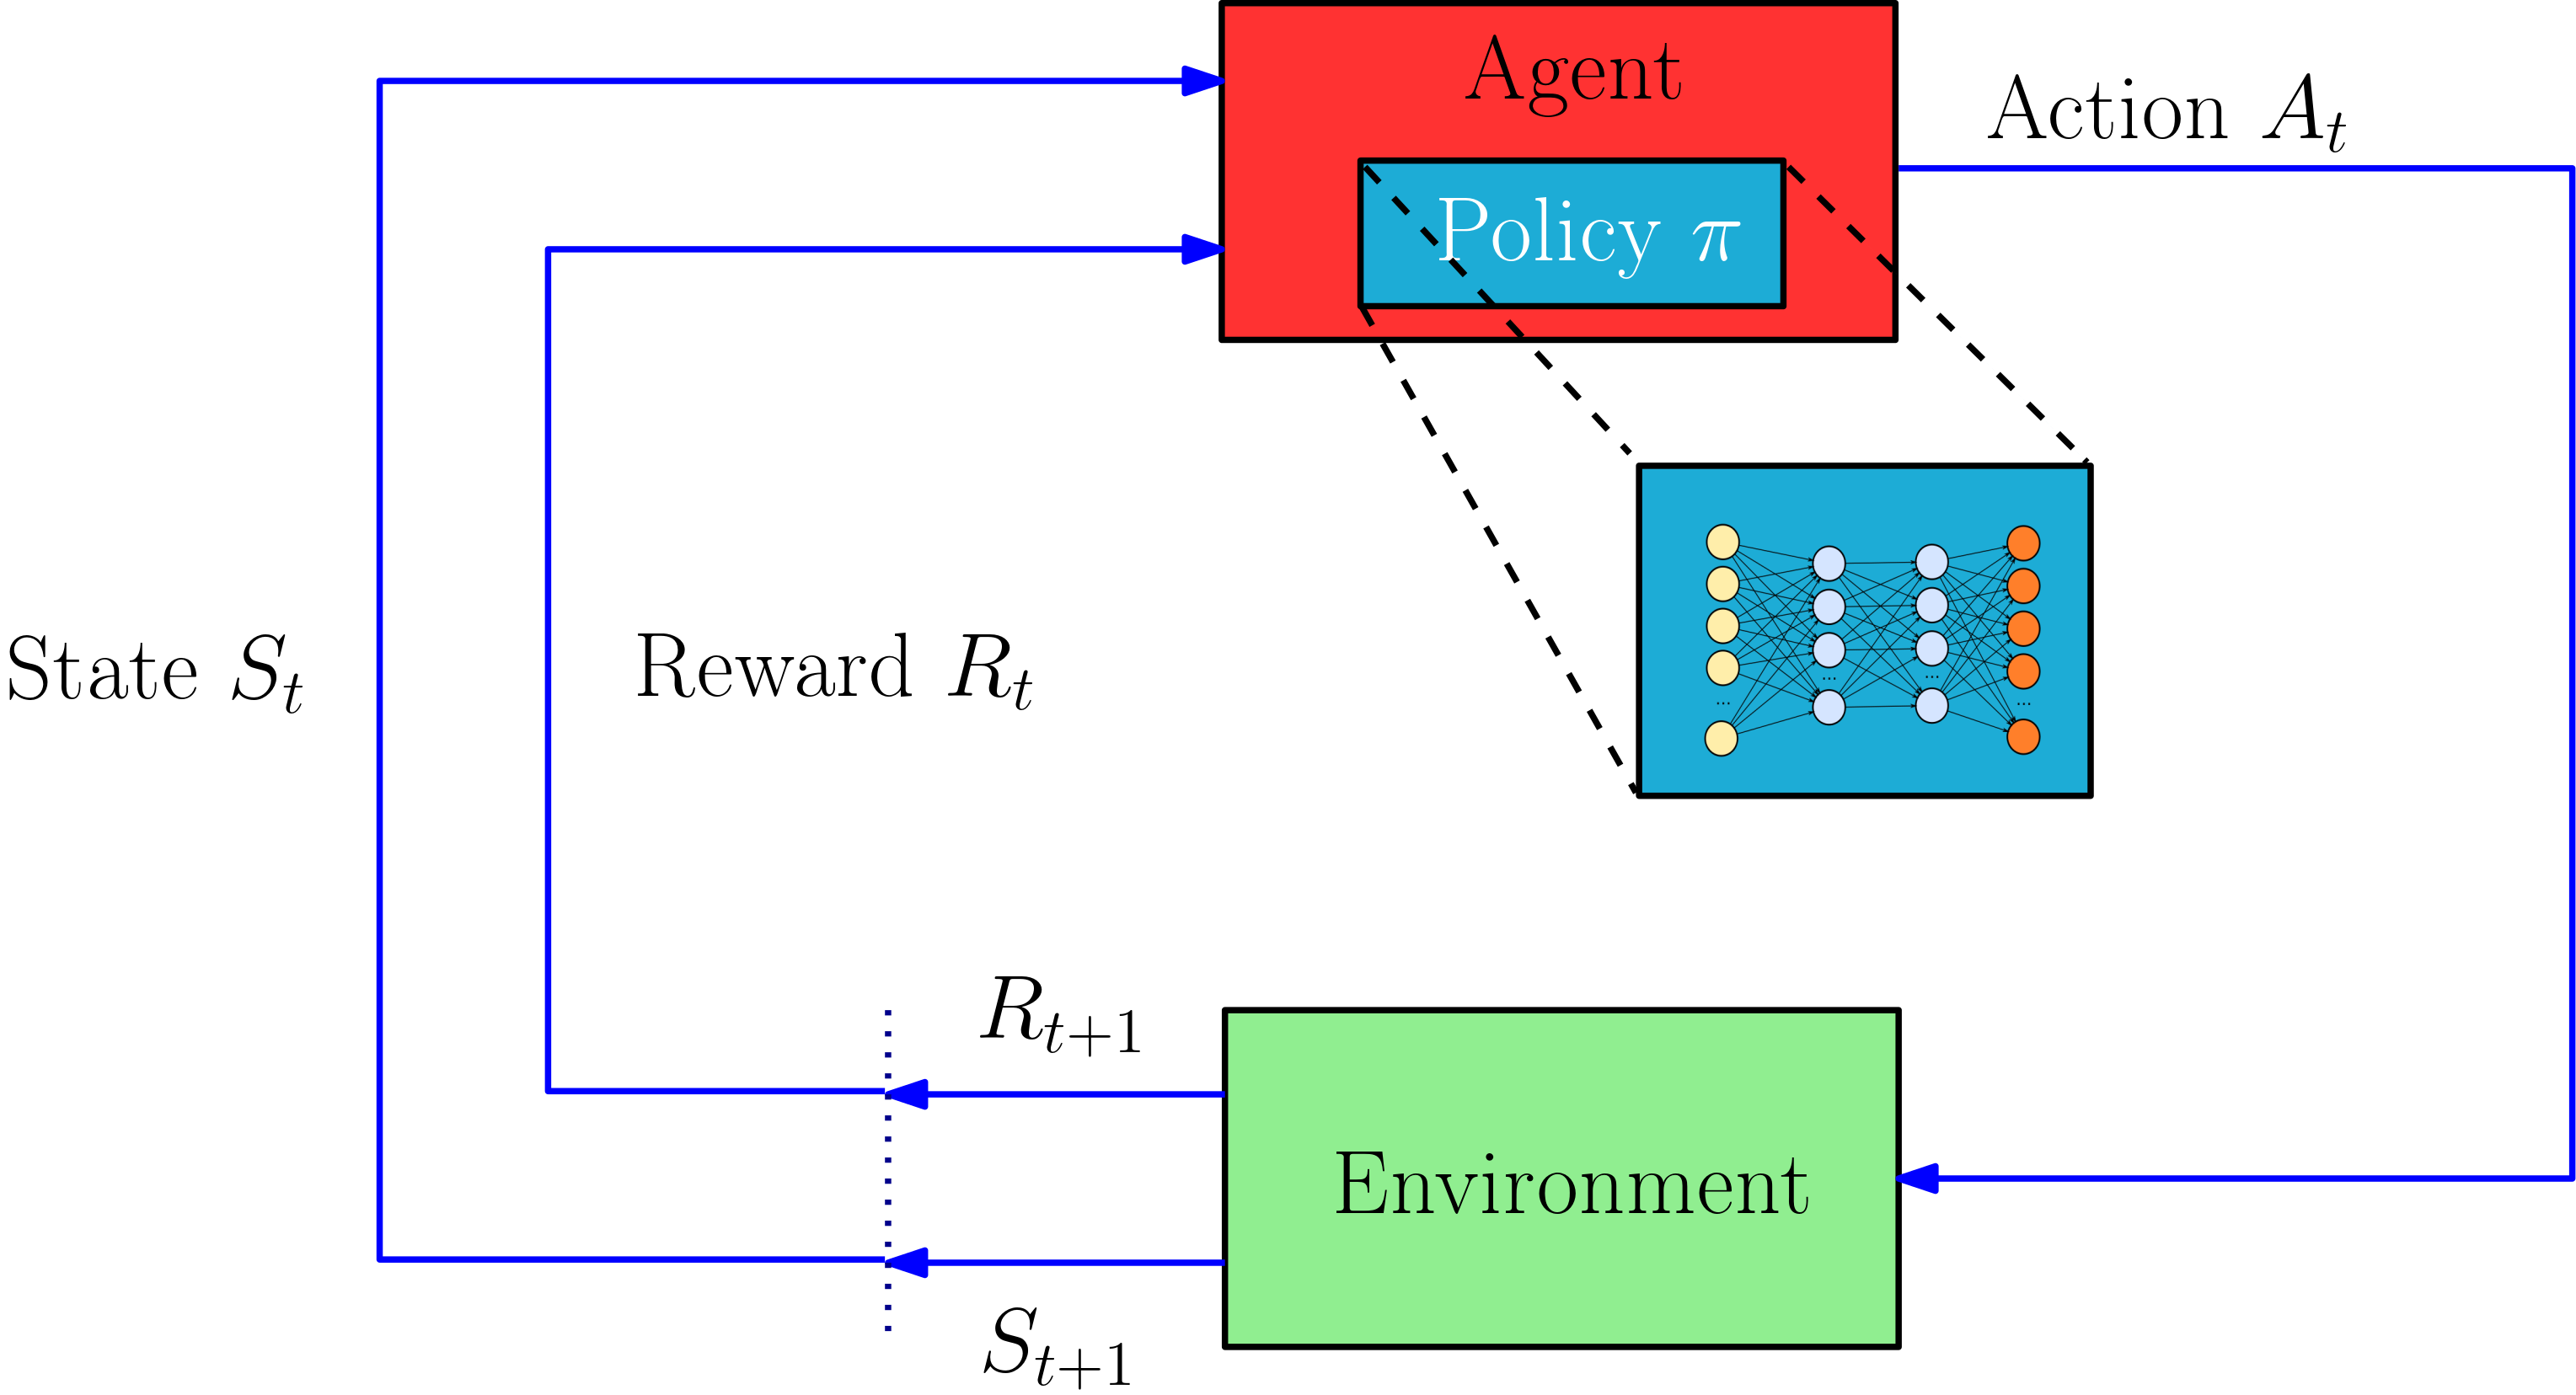
\includegraphics[width=0.9\textwidth]{images/drlv3.png}
    \caption{Deep Reinforcement Learning}
    \label{fig:rl}
\end{figure}

\section{TRANSFER LEARNING}

Transfer learning is a method that improves the performance
on the target task by leveraging the knowledge gained by
performing the same experiment on a similar source task. This
can be often seen in supervised learning problems such as
image labeling, where the knowledge from the source task is
used to enhance the performance and efficiency of learning in
the target task. However, this can be quite challenging in
reinforcement learning, as each problem may have a different
state space. We are able to utilize transfer learning to
learn tasks that are rather similar, i.e, having a similar
observation space and states.

\begin{figure}[H]
    \centering
    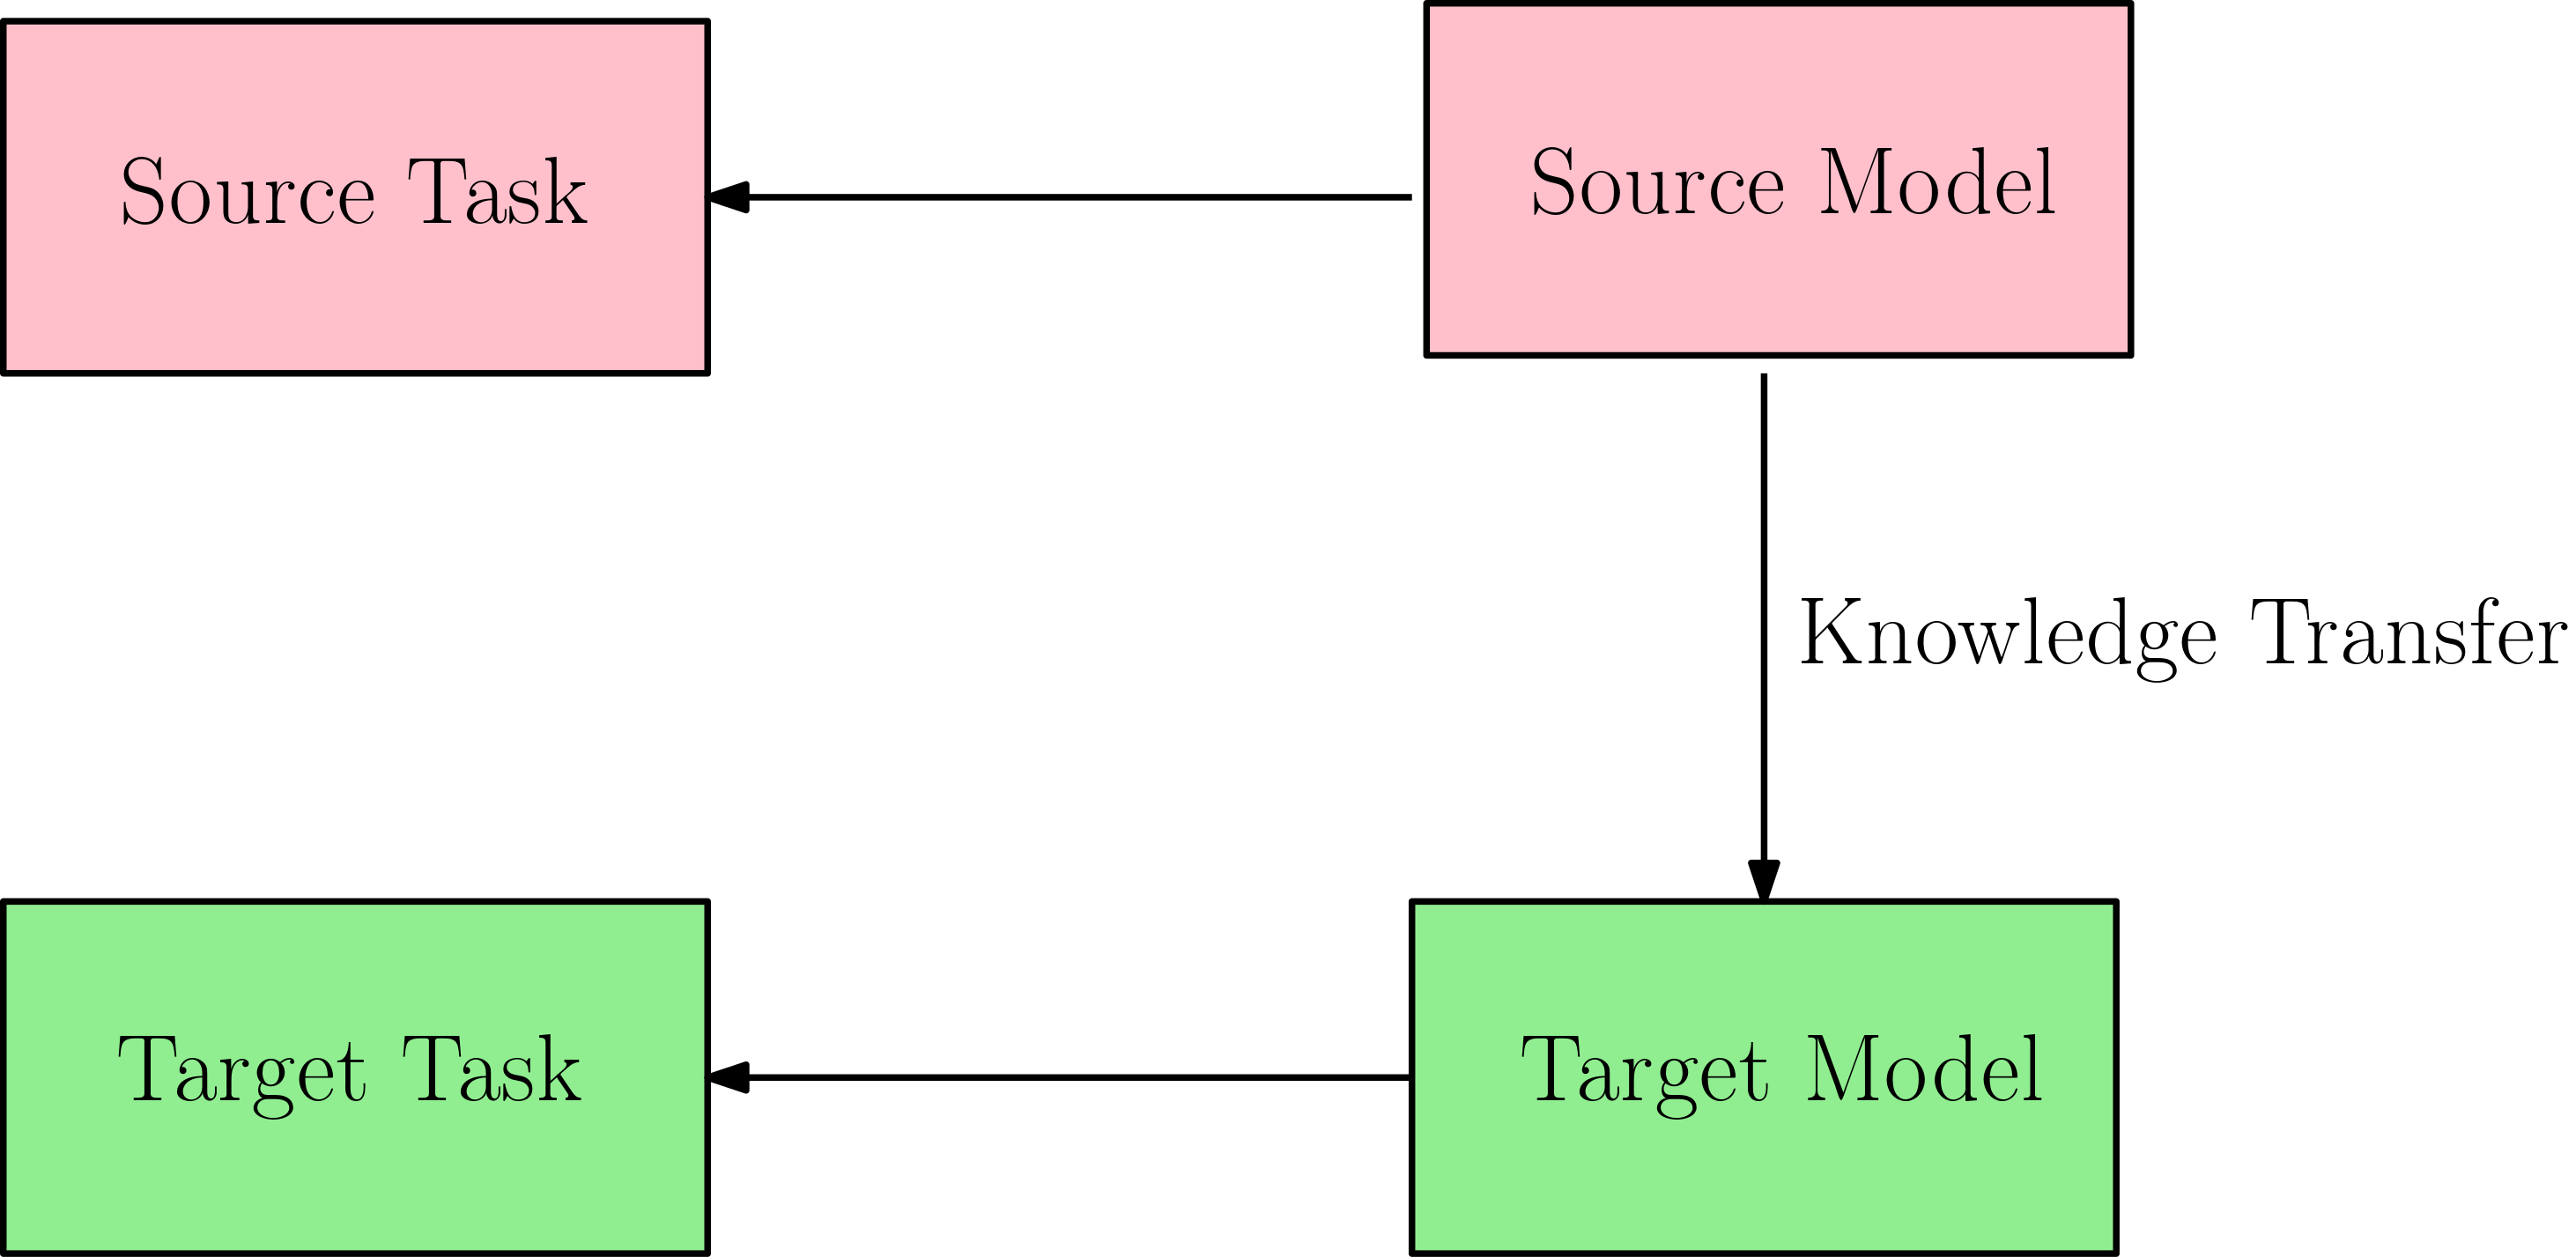
\includegraphics[width=0.9\textwidth]{images/tlv3.png}
    \caption{Transfer Learning}
    \label{fig:rl}
\end{figure}

\section{ADVERSARIAL TRAINING}

Many machine learning and deep learning models are often
trained and tested on data from the same statistical
distribution, and are hence often overtuned to perform well
only on said distribution. This however causes issues when
deployed with real world data and may be prone to adversaries
that may take advantage of this fact and compromise the
result of the model. Thus we use adversarial training to
mitigate this concern.

Adversarial training in reinforcement learning is made
possible by using an adversary to attack the observations or
the actions of the model. Knowing that adversarial training
improves representational learning in supervised models, we
can intuitively say that using adversarial training along
with transfer learning will improve the performance of an
agent using reinforcement learning.

\begin{figure}[H]
    \centering
    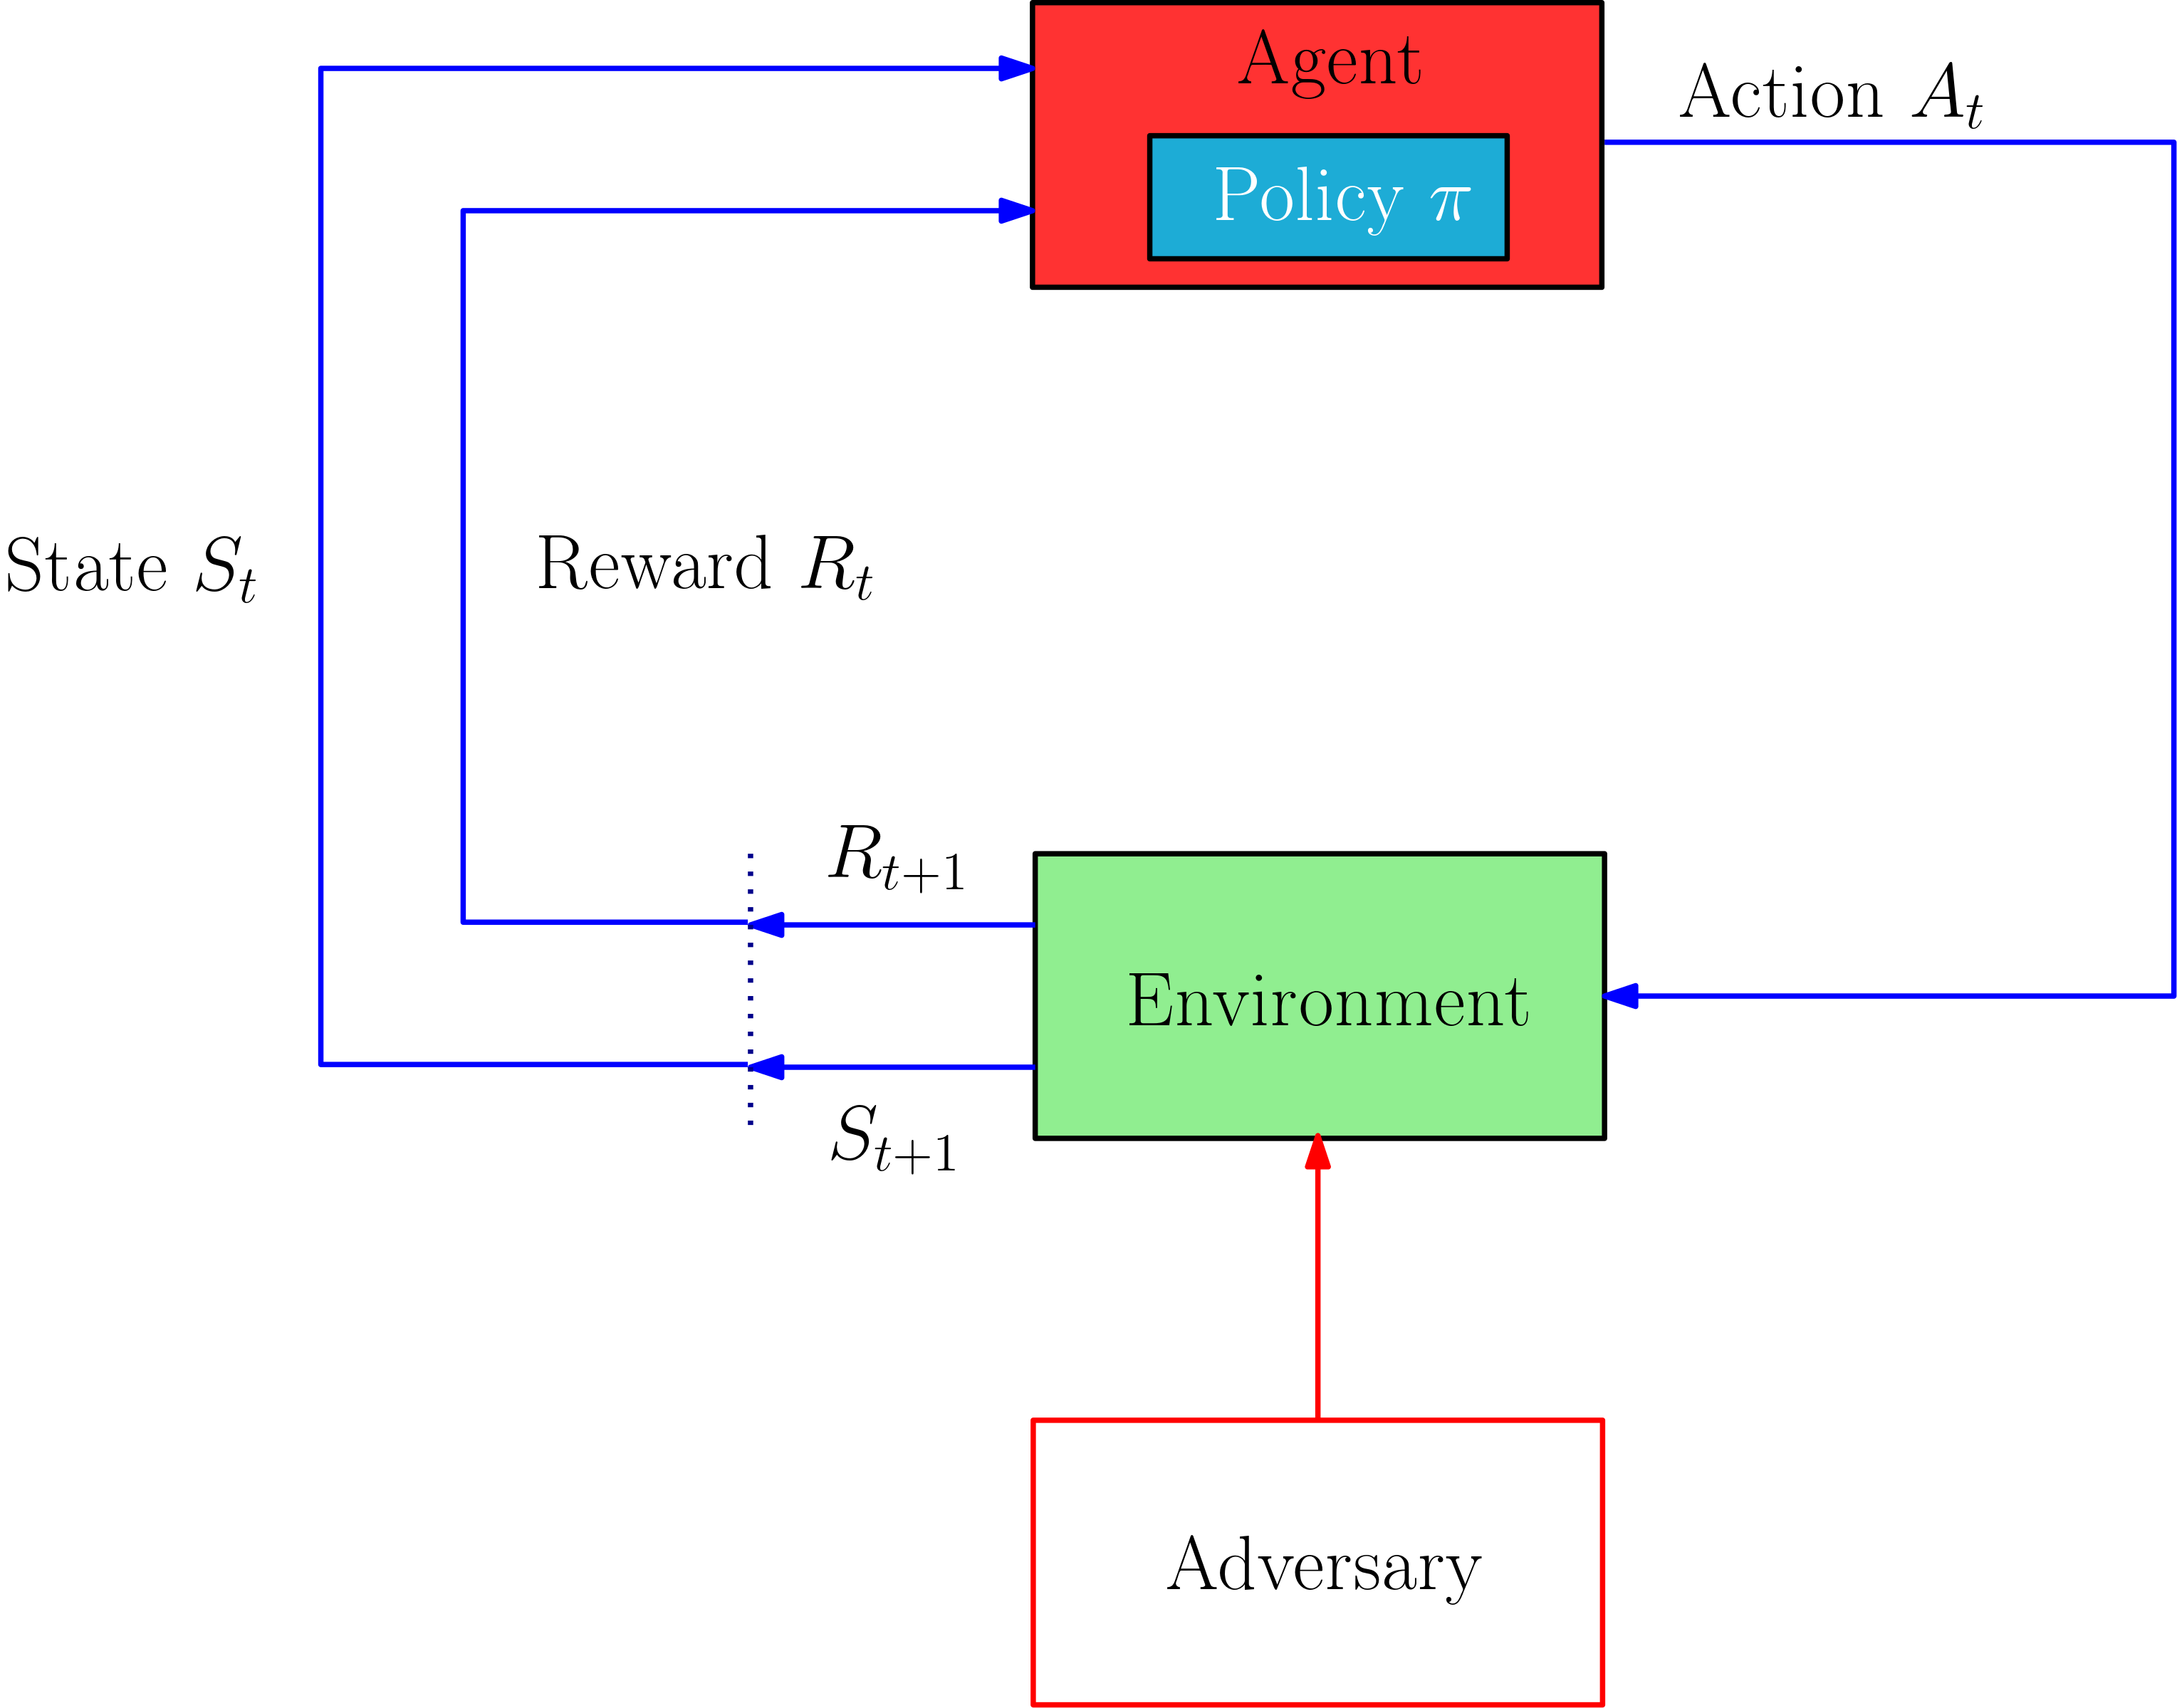
\includegraphics[width=0.9\textwidth]{images/rl_atv3.png}
    \caption{Adversarial Training in Reinforcement Learning}
    \label{fig:rl}
\end{figure}

\section{UNITY}

Unity is the game engine used to create
environments. Unity allows us to create a 3D environment on
which we can run our reinforcement learning algorithms. It
uses a scripting API written in C\#. The engine also supports
Object Oriented Programming paradigm, to create various game
objects components that enable us to create an interactive
environment for our agent.

Unity provides the user with a console, in which we can
visualize the various components of the environments. The
properties and functionalities of said components are defined
in their respective script files. This gives us great control
over the environment. We can set the goal state of the agent
and define the various events on which we give the agent a
reward; this is done by calling the API provided by
unity. This flexibility in defining the problem makes Unity
all the more alluring and our primary choice for creating an
environment.

Unity provides a package known as MLagents which provides a
wrapper API and some baseline implementations of well known
Deep Reinforcement learning algorithms. It also acts as the
connector between the model and the environment enabling us
to configure different models and train them in our
environment.

